\documentclass[oneside,final,14pt,a4paper]{extreport}

% custom
\usepackage[table]{xcolor}
\usepackage{geometry}
\usepackage{todonotes}

\usepackage{algorithm}
\usepackage{algpseudocode}
\usepackage{tabularx}

\usepackage{siunitx}
\usepackage{numprint}

\usepackage{makecell}
% custom

\usepackage{tempora} % Times New Roman alike font  


\usepackage{vmargin}
\setpapersize{A4}
\setmarginsrb{2.5cm}{2.0cm}{2.0cm}{2.0cm}{0pt}{10mm}{0pt}{13mm}
\usepackage{setspace}
\setstretch{1.5}
\usepackage{indentfirst}
\parindent=1.25cm

%%%%% ADDED TO SUPPORT TT BOLD FACES %%%%
\DeclareFontShape{OT1}{cmtt}{bx}{n}{<5><6><7><8><9><10><10.95><12><14.4><17.28><20.74><24.88>cmttb10}{}
\renewcommand{\ttdefault}{pcr}
%%%%% END %%%%%%%%%%%%%%%%%%%%%%%%%%%%%%% 

\usepackage{atbegshi,picture}
\usepackage[T1,T2A]{fontenc}
\usepackage[utf8]{inputenc}

\usepackage[english,russian]{babel}
\usepackage[backend=biber,style=ieee,autocite=inline]{biblatex}
\bibliography{ref.bib}
\DefineBibliographyStrings{russian}{%
  bibliography = {References},}
\usepackage{blindtext}

\usepackage{pdfpages}
\newenvironment{bottompar}{\par\vspace*{\fill}}{\clearpage}
\usepackage{amsmath,amsfonts}
\usepackage{url}
\usepackage{amsthm}
\newtheorem{theorem}{Theorem}
\newtheorem{corollary}{Corollary}
\newtheorem{lemma}{Lemma}
\newtheorem{proposition}{Proposition}
\theoremstyle{definition}
\newtheorem{definition}{Definition}
\theoremstyle{remark}
\newtheorem*{remark}{Remark}
\theoremstyle{remark}
\newtheorem*{example}{Example}

\usepackage{float}
\usepackage{graphicx}
\graphicspath{{figs/}} %path to images
\usepackage{array}
\usepackage{multirow,array}
\usepackage{caption}
\usepackage{subcaption}
\usepackage{hyperref}
\hypersetup{colorlinks=true, linkcolor=black, citecolor=black}
\usepackage{paralist}
\usepackage{listings}
\usepackage{zed-csp}
\usepackage{fancyhdr}
\usepackage{csquotes}
% \usepackage{anyfontsize}
% \usepackage{mathptmx}
% \usepackage{t1enc}

\usepackage{chngcntr}
\usepackage{upgreek} 
\usepackage{bm}
\usepackage{booktabs}
\usepackage{multirow}
\usepackage{longtable}
\usepackage[font=singlespacing, labelfont=bf]{caption}
%Hints
\newcommand\pic[1]{(Fig. \ref{#1})} %Ref on figure
\newcommand\tab[1]{(Tab. \ref{#1})} %Ref on table

\setlength{\headheight}{32.0976pt}
\usepackage{enumitem}
\newlist{inlinelist}{enumerate*}{1}
\setlist*[inlinelist,1]{%
  label=(\arabic*),
}

% \setcounter{secnumdepth}{4}
\captionsetup[table]{labelfont={normalfont}, name={TABLE}, labelsep={newline}}
\setlength{\parindent}{2em} 
\DeclareCaptionLabelSeparator{figSep}{.\quad}
\captionsetup[figure]{labelfont={normalfont}, name={Fig.}, labelsep=period}
\counterwithin{figure}{chapter}

\usepackage{titlesec}
\titleformat{\chapter}[display]
  {\normalfont\huge\bfseries}       % стиль шрифта
  {Глава \thechapter}             % формат нумерации
  {0pt}                             % вертикальный отступ между "Chapter X" и заголовком
  {\vspace{0pt}}                    % отступ перед заголовком
\titlespacing*{\chapter}{0pt}{0pt}{6pt}  % отступ до и после

% \titleformat{\section}[hang]{\fontsize{20}{24}\selectfont\filcenter}{\Roman{section}}{1em}{}
% \titleformat{\subsection}[hang]{\itshape}{\Alph{subsection}.}{1em}{}[]
% \titleformat{\subsubsection}[runin]{\itshape}{\arabic{subsubsection})}{1em}{}[$:$]
% \titlespacing{\subsubsection}{1em}{1em}{1em}
% \titleformat{\paragraph}[runin]{\itshape}{\alph{paragraph})}{1em}{}[$:$\quad]
% \titlespacing{\paragraph}{2em}{1em}{1em}

\usepackage{placeins} % for \FloatBarrier

\pagestyle{fancyplain}

% remember section title
\renewcommand{\chaptermark}[1]%
	{\markboth{\chaptername~\thechapter~--~#1}{}}

% subsection number and title
\renewcommand{\sectionmark}[1]%
	{\markright{\thesection\ #1}}

\rhead[\fancyplain{}{\bf\leftmark}]%
      {\fancyplain{}{\bf\thepage}}
\lhead[\fancyplain{}{\bf\thepage}]%
      {\fancyplain{}{\bf\rightmark}}
\cfoot{} %bfseries


\newcommand{\dedication}[1]
   {\thispagestyle{empty}
     
   \begin{flushleft}\raggedleft #1\end{flushleft}
}

\addto\captionsenglish{\renewcommand{\contentsname}{Оглавление}}

\begin{document}

% tables
\definecolor{lightgray}{gray}{0.95}
% \rowcolors{2}{white}{lightgray}
% tables

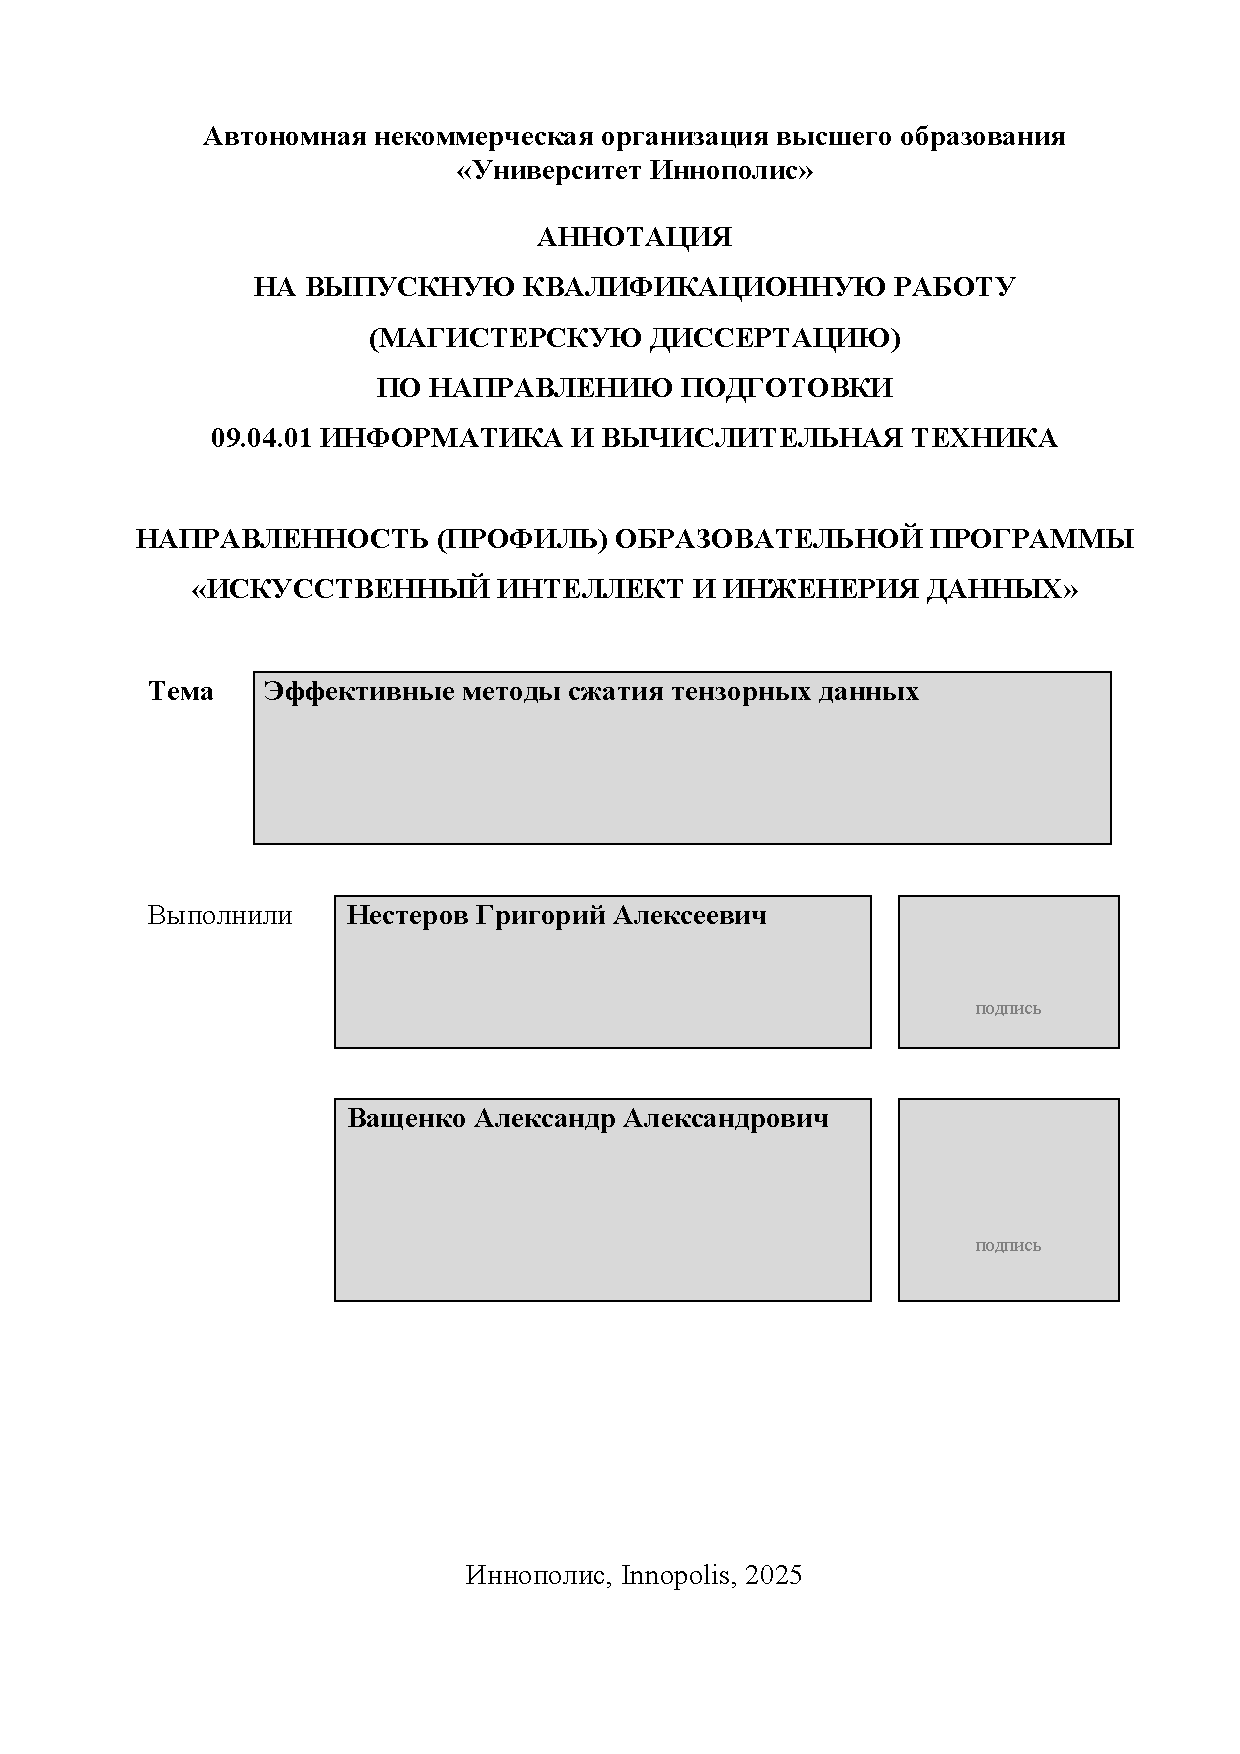
\includepdf[pages=-, offset=2.5cm -2.0cm]{title.pdf}
\tableofcontents
\newpage


\setcounter{page}{3}

% введение
\chapter{Введение}
\label{chap:intro}

\chaptermark{Введение}

Высокоразмерные данные (тензоры) встречаются в различных прикладных областях. В качестве примеров могут выступать: нейронные сети, медико-биологические сигналы (ЭЭГ, МРТ), гиперспектральных изображений. Такие данные становятся все больше, требуя больших вычислительных мощностей для их использования. Классические методы тензорной декомпозиции, такие как Tucker~\cite{tensorly_parafac_tucker}, Tensor-Train (TT)~\cite{tensorly_tensor_train}, CANDECOMP/PARAFAC (CPD/CP)~\cite{tensorly_parafac_tucker, tensorly_parafac_2, tensorly_parafac_3, tensor_decompositions_for_data_science, tensor_computation_for_data_analysis}, и их современные расширения позволяют аппроксимировать исходные тензора, уменьшая требуемый объём памяти и ускоряя вычисления на получаемых структурах~\cite{tensor_decompositions_for_data_science, tensor_computation_for_data_analysis}. Однако эффективность разложения сильно зависит от правильно выбранных параметров метода, самого метода декомпозиции, что остаётся открытой исследовательской проблемой в зависимости от метода декомпозиции.

\textbf{Актуальность работы.} С ростом масштабов нейронных сетей и объёмов научных данных возрастает потребность в универсальных, устойчивых и масштабируемых методах тензорного сжатия, которые предоставляют гарантированное качество аппроксимированных данных и имеют готовые реализации с низкими накладными расходами по времени и памяти.

\textbf{Цель работы} — разработать и экспериментально обосновать эффективные методы выбора ранга и практические рекомендации по применению методов тензорной декомпозиции на примере задачи тензорного сжатия. А также в качестве прикладного практического примера, воспроизвести и улучшить, на основе существующего исследования, метод сжатия нейронных сетей.

\textbf{Задачи работы:}
\begin{enumerate}
  \item Провести теоретический и эмпирический анализ распространённых методов тензорной декомпозиции (Tucker, TT, CPD, RTPCA~\cite{rtpca_method}) на тензорах примерах: изображения (3D), видео (4D) и ЭЭГ (6D).  
  \item Сравнить современные Python-библиотеки по метрикам «время исполнения», «пиковое потребление памяти» и «норма Фробениуса ошибки восстановления».  
  \item Разработать алгоритм автоматического выбора ранга для форматов Tucker и TT, обеспечивающий заданное отношение сжатия при минимальной ошибке.  
  \item Интегрировать алгоритм в конвейер сжатия сверточных и полносвязных слоёв и предоставить открытый Python-код.  
  \item Оценить точность–сжатие на стандартных архитектурах CNN и выделить направления дальнейшей оптимизации.
\end{enumerate}

\textbf{Научная новизна} работы заключается в предложении адаптивной процедуры выбора ранга, позволяющей автоматически контролировать компромисс «точность–компрессия» для неоднородных тензоров и слоёв нейронных сетей.  

\textbf{Практическая значимость.}  
Разработанный программный пакет и методические рекомендации облегчают выбор инструментария при применении тензорных разложений в прикладных задачах хранения, передачи и ускорения обработки данных.  

В дальнейших разделах аннотации последовательно рассмотрены исходные предпосылки, методология экспериментов, полученные результаты и выводы, что отражает структуру магистерской диссертации.


% терминология
\chapter{Обзор литературы}
\label{chap:lr}
\chaptermark{Обзор литературы}


% обзор литературы
\chapter{Обзор литературы}
\label{chap:lr}
\chaptermark{Обзор литературы}

В справочной части диссертации проанализированы четыре ключевые семьи тензорных разложений: \emph{CANDECOMP/PARAFAC} (CP), \emph{Tucker} (HOSVD), \emph{Tensor-Train} (TT) и \emph{Robust Tensor PCA} (RTPCA) как представитель устойчивых методов. Рассмотрены их математические основы, недавние усовершенствования и практические сценарии использования.

\subsection*{Классический инструментарий}

\begin{itemize}\setlength\itemsep{0.25em}
    \item \textbf{CP-разложение} (Hitchcock 1927; Carroll \& Chang 1970) аппроксимирует тензор суммой рангов-1, обеспечивая структурную интерпретируемость при условной уникальности представления. Основные проблемы: выбор ранга \(R\) и вычислительная устойчивость для высоких порядков.
    \item \textbf{Tucker/HOSVD} (Tucker 1966) разлагает тензор на компактное ядро \( \mathcal{G} \) и матрицы факторов \(\{A_n\}\) со свободными рангами \(R_n\) по модам. Гибкость даёт высокую точность и возможности денойзинга, но порождает неоднозначность факторов и сложность подбора рангов.
    \item \textbf{Tensor-Train (TT)} (Oseledets 2011) хранит данные цепочкой ядер и TT-рангов, переводя экспоненциальную сложность в линейную по порядку \(d\). Метод широко применяется для сжатия параметров нейросетей и решения многомерных уравнений.
\end{itemize}

\subsection*{Устойчивые и современные расширения}

\begin{itemize}\setlength\itemsep{0.25em}
    \item \textbf{Robust Barron-Loss Tucker} \cite{barron_loss_tensor_decomposition} заменяет норму Фробениуса обобщённой Barron-функцией, уменьшая влияние выбросов при сохранении управляемости гладкостью.
    \item \textbf{RTPCA} \cite{rtpca_method} сочетает ядерную норму и $\ell_1$-штраф для разделения низкоранковой структуры и разреженных выбросов. Эффективна в видео-денойзинге и медицинских данных.
\end{itemize}

\subsection*{Прикладные тенденции}

\begin{itemize}\setlength\itemsep{0.25em}
    \item \textbf{Компрессия CNN.}  
    \emph{Stable Low-rank Decomposition} \cite{stable_low_rank_tensor_decomposition} объединяет CP и Tucker для фильтров 3\(\times\)3 (VGG-16, ResNet-18), достигая лучшего баланса «точность–ускорение».  
    \emph{Hybrid TT + Hierarchical Tucker} \cite{hybrid_tensor_decomposition_c_nn} показывает, что разные форматы оптимальны для свёрточных и полносвязных слоёв соответственно.
    \item \textbf{Оптимизационные фреймворки.}  
    Работы \cite{yin2021efficienttensordecompositionbaseddnn} объединяют ADDM-регуляризацию, TT-разложение и дообучение, позволяя либо повысить точность, либо добиться экстремальных коэффициентов сжатия.
    \item \textbf{Масштабируемые аппроксимации.}  
    \emph{Cross Tensor Approximation} (CTA) \cite{cross_tensor_approximation} обходит полную SVD, используя выборку срезов/фибр и малое ядро; обеспечивает скорость и малый объём памяти для гиперспектральных и EEG-тензоров.
    \item \textbf{Временная разреженность.}  
    Time-aware разложения \cite{time_aware_tensor_decomposition} вводят динамический штраф по временной моде, сочетая аналитическое и итеративное обновления матриц факторов для эволюционирующих данных.
\end{itemize}

\subsection*{Выводы и выявленные пробелы}

Обзор показывает, что:

\begin{enumerate}\setlength\itemsep{0.25em}
    \item Выбор ранга остаётся главным фактором влияния на компромисс «точность–степень сжатия» и не решён универсально для Tucker и TT.  
    \item Современные библиотеки (TensorLy, tntorch, T3F и др.) различаются по API-зрелости и производительности; нет независимого бенчмарка, охватывающего 3D–6D тензоры разных типов.  
    \item Робастные формулировки (Barron-Loss, RTPCA) улучшают устойчивость, но требуют специализированных процедур ранжирования и ещё мало интегрированы в софт для нейросетей.
\end{enumerate}

Эти пробелы мотивируют практические задачи диссертации: (i) построить единый бенчмарк библиотек, (ii) разработать автоматический выбор ранга для Tucker и TT под заданное отношение сжатия, (iii) внедрить алгоритм в конвейер сжатия слоёв CNN и провести эмпирическую оценку.
% методология
\chapter{Методология}
\label{chap:methodology}
\chaptermark{Методология}

В данной главе описывается структура бенчмарка и представлены количественные критерии оценки методов тензорного разложения, включающие:
\begin{itemize}
    \item использование памяти различными компонентами вычислений,
    \item ошибку Фробениуса,
    \item время вычислений.
\end{itemize}
Рассматриваются типы тензорных данных, особенности их представления, а также процедуры выбора параметров разложения. Особое внимание уделяется методам оптимизации ранга для разложений Тукера и Тензорного Поезда (Tensor Train, TT). Также описан алгоритм сжатия нейронных сетей и внедрённые улучшения.

\section{Типы тензорных данных для бенчмарка}
\label{sec:tensor_data_types_for_benchmark}

В этой секции представлены используемые типы тензорных данных и их конкретные примеры, применяемые для оценки и сравнения методов и библиотек тензорного разложения. Примеры демонстрируют возможности и сферу применения методов разложения.

\subsection*{Изображения}

Изображения представлены трёхмерными тензорами с размерами, соответствующими высоте, ширине и цветовым каналам (RGB). Данные загружаются из распространённых форматов (jpg, png) с помощью библиотеки OpenCV-Python.

Для бенчмарка выбраны три варианта изображений с разными размерами и аспектами:
\begin{itemize}
    \item среднее изображение с размером (564, 564, 3),
    \item изображение с другим соотношением сторон (412, 620, 3),
    \item крупное изображение с высоким разрешением (689, 1195, 3).
\end{itemize}

Такие данные позволяют оценить влияние размера, соотношения сторон и цветовой палитры на качество и производительность методов тензорного разложения.

\subsection*{Видео}

Видео рассматриваются как четвёртого порядка тензоры \(\mathcal{X} \in \mathbb{R}^{T \times H \times W \times 3}\), где \(T\) — число кадров, \(H\) и \(W\) — высота и ширина кадра соответственно, 3 — количество цветовых каналов RGB.

Для бенчмарка выбраны три видеоролика с различной длительностью и пространственным разрешением, загруженные с YouTube и обработанные через OpenCV-Python. Выбор сделан с учётом ограничения вычислительных ресурсов, чтобы обеспечить воспроизводимость экспериментов.

\subsection*{ЭЭГ (электроэнцефалография)}

Для тестирования методов на тензорах высокого порядка использованы два набора данных ЭЭГ:

\begin{itemize}
    \item \textbf{EEG Motor Movement/Imagery Dataset} \cite{Schalk2004BCI2000} — шестимерный тензор с размерностями, отражающими субъектов, запуски экспериментов, типы событий, эпизоды, каналы и временные отсчёты. Использованы данные четырёх субъектов и двенадцати запусков для сохранения вариативности и управляемости вычислений.
    \item \textbf{LIMO dataset} — данные, доступные в библиотеке MNE-Python, содержащие тензор с пятью измерениями, включающими субъектов, запуски, испытания, события и временные отсчёты. Размеры были усечены до общих для всех субъектов значений для обеспечения однородности.
\end{itemize}

\section{Оптимальный выбор ранга для разложений Тукера и Tensor Train}
\label{sec:rank_selection_methodology}

Выбор ранга является ключевым в тензорных разложениях, так как определяет компромисс между степенью сжатия и ошибкой аппроксимации. Задача формулируется как ограниченная задача оптимизации, решаемая с помощью локальных и глобальных алгоритмов минимизации из пакета \texttt{SciPy} с использованием разложений из \texttt{TensorLy}.

\subsection*{Ограничения на ранги}

\paragraph{Tensor Train.} Для каждого внутреннего ранга \(r_k\) действуют классические ограничения:
\[
1 \le r_k \le \min\left(\prod_{i=1}^k I_i,\; \prod_{j=k+1}^N I_j\right), \quad k=1,\dots,N-1,
\]
где \(\mathcal{X} \in \mathbb{C}^{I_1 \times \dots \times I_N}\) — исходный тензор, \(I_k\) — размерность \(k\)-го моды, \(r_k\) — \(k\)-й TT-ранг, \(N\) — порядок тензора. Внешние ранги фиксированы: \(r_0 = r_N = 1\).

\paragraph{Tucker.} Для разложения Тукера ранги выбираются для каждого измерения:
\[
1 \le r_n \le I_n, \quad n=1,\dots,N,
\]
где \(r_n\) — ранг Тукера вдоль \(n\)-й моды.

\subsection*{Функция потерь}

Для каждой комбинации рангов строится приближение исходного тензора, после чего оцениваются два параметра:

\begin{enumerate}
    \item Относительная ошибка Фробениуса — отношение нормы разности исходного и приближённого тензоров к норме исходного.
    \item Коэффициент сжатия — отношение объёма памяти, занимаемого факторами разложения, к объёму памяти исходного тензора.
\end{enumerate}

Оптимизация сводится к поиску рангов, минимизирующих комбинацию этих показателей с учётом баланса между точностью и сжатием.

\section{Сжатие нейронных сетей}

Для демонстрации практического применения методов тензорного разложения реализован алгоритм сжатия сверточной нейронной сети. Внедрены улучшения, направленные на повышение эффективности сжатия без существенной потери качества.

---

Таким образом, методология включает разработку комплексного бенчмарка, описывающего разнообразные типы данных, строгие критерии оценки и алгоритмические подходы к оптимальному выбору ранга в задачах тензорного сжатия и аппроксимации.

% реализация
\chapter{Анализ Результатов}
\label{chap:eval}
\chaptermark{Анализ результатов}


% анализ результатов
\chapter{Анализ результатов}
\label{chap:eval}
\chaptermark{Анализ результатов}

В данном разделе представлен сравнительный анализ эффективности различных методов оптимизации рангов тензорных разложений, а также оценка производительности популярных библиотек для работы с тензорами.

Исследование показало, что локальные градиентные методы, такие как Nelder–Mead и SLSQP, продемонстрировали низкую адаптивность при поиске оптимальных рангов. В частности, они часто сходились к начальному низкорейтинговому решению [1,1,1,1], что указывает на их склонность к застреванию в локальных минимумах без возможности выхода. Это обусловлено многомодальностью и дискретной природой пространства рангов, а также отсутствием механизма глобального поиска. Таким образом, применение указанных алгоритмов требует существенной модификации или гибридизации с эвристическими методами для повышения качества оптимизации.

Скорость работы методов была оценена отдельно: SLSQP оказался наиболее быстрым, однако качество найденных решений было наихудшим. Это подчёркивает известный компромисс между быстродействием и точностью в задачах оптимизации рангов.

Из рассмотренных глобальных методов Grid Search и Random Search проявили себя менее эффективно с точки зрения времени выполнения, однако обеспечивали более устойчивый поиск, что соответствует их полной или частичной переборной природе. Предложенный автором метод Coordinate Descent, дополненный локальной оптимизацией, продемонстрировал наилучшее сочетание качества решения и приемлемого времени работы.

Сравнение библиотек TensorLy, TensorFlow, и tntorch выявило, что TensorLy обеспечивает наиболее быструю и стабильную работу на тестовых тензорах с малыми и средними размерностями. TensorFlow показал высокую производительность на крупных тензорах благодаря GPU-ускорению, но страдал от повышенного потребления памяти. Библиотека tntorch оказалась самой медленной, что обусловлено спецификой реализации и отсутствием эффективной поддержки некоторых видов разложений.

Анализ логов экспериментов подтвердил критическую важность тщательного выбора стратегии оптимизации рангов для достижения компромисса между точностью восстановления тензора и вычислительными затратами. Результаты указывают на необходимость разработки более адаптивных и гибридных алгоритмов, способных учитывать специфику задачи и структуру данных.

Таким образом, проведённое исследование выявило ключевые ограничения существующих методов и библиотек, а также продемонстрировало перспективность предложенного подхода на основе локального и глобального поиска с комбинированием эвристик. Это открывает возможности для дальнейших разработок в области эффективного сжатия и анализа многомерных данных.


% заключение
\chapter{Заключение}
\label{chap:conclusion}
\chaptermark{Заключение}

Работа обобщает результаты систематического исследования тензорных разложений для трёх классов данных (изображения, видео и ЭЭГ) и их применения к сжатию глубинных нейросетей. Решены все поставленные в начале задачи.

\textbf{Основные достижения.}
\begin{enumerate}\setlength\itemsep{0.3em}
    \item \emph{Качественный обзор} \,> 30 библиотек; сформирован краткий «шорт-лист» Python-инструментов (TensorLy, T3F), пригодных для воспроизводимых экспериментов.
    \item \emph{Бенчмарк 10 000+ прогонов} на 3D–6D тензорах: измерены время, пиковая RAM/VRAM и ошибка Фробениуса. Выявлено, что TensorLy-TT обеспечивает оптимальный баланс точности и ресурсов; даны практические настройки гиперпараметров для CP, Tucker и TT.
    \item Разработан \emph{автоматический выбор ранга} для форматов Tucker и Tensor-Train. Алгоритм на базе дифференциальной эволюции гарантирует заданное сжатие (50 \%) при минимальной ошибке; опубликован модуль \texttt{rank\_search}.
    \item Воссоздан и улучшен \emph{конвейер сжатия CNN}. Для VGG и ResNet получено 4–8x уменьшение параметров и 14–22 \% ускорение инференса при падении Top-1 не более 1 pp (часто — рост после fine-tuning).
\end{enumerate}

\textbf{Практическая ценность.}
\begin{itemize}\setlength\itemsep{0.25em}
    \item Открытый репозиторий содержит полный код, журналы и ноутбуки (\url{https://github.com/Innopolis-tensor-compression/tensor-compression-methods}), обеспечивая воспроизводимость и возможность дальнейшего расширения.
    \item Рекомендации по выбору библиотек, форматов и параметров пригодны для прикладных задач хранения, передачи и ускорения моделей и многомерных данных.
\end{itemize}

\textbf{Ограничения и направления будущих работ.}
\begin{itemize}\setlength\itemsep{0.25em}
    \item Улучшить функцию потерь и исследовать гибридные «глобальный + локальный» оптимизаторы ранга.
    \item Расширить конвейер на другие типы слоёв (групповые свёртки, attention) и форматы (Tensor Ring).
    \item Дополнить бенчмарк новыми наборами данных (аудио, гиперспектр) и библиотеками (EXATN, Scikit-TT).
\end{itemize}

Таким образом, работа вносит вклад в практику эффективного сжатия тензорных данных и моделей, предлагая как новые алгоритмы, так и документированную инфраструктуру для их оценки и применения.


%% REFERENCES
\printbibliography[heading=bibintoc,title={Список литературы}]
\include{chapters/appex}
\end{document}